\documentclass{beamer} 
%\documentclass[handout]{beamer} 

% Michael Maier, 2014.
% CC-BY-SA 3.0 at

\usepackage[utf8]{inputenc}
\usepackage[ngerman]{babel}

\title{OpenStreetMap - Die freie Weltkarte} 
\author{Michael Maier \textless Michael.Maier@student.tugraz.at\textgreater} 
\date{27. November 2014} 

\usetheme{Antibes}

\hypersetup{colorlinks=true,urlcolor=blue,linkcolor=white}

%\usebackgroundtemplatei{
%
\includegraphics[width=\paperwidth,
%height=0.8\paperheight]{mag_map.png}
%}

\begin{document}

%\maketitle

\begin{frame} 


\begin{figure}
  \centering
  
\includegraphics[width=.5\textwidth]{mag_map.png}
\end{figure}

\begin{center}
\Huge{OpenStreetMap\\}
\end{center}

\begin{center}
\Large{\emph{Die freie Weltkarte}}
\end{center}

\end{frame}


% Zielgruppe
% * Politiker, um die 60 ohne jedes technische Wissen

% tolle Bilder herzeigen!
% * irgendein Zoo
% * 3D
% * Tolle Kartenstile:
%     * OSM-Fr?
%     * stamen watercolor
%     * pistemap
%     * bicycle map
%     * OpenSeaMap
%
% Dokumentation (nenne es doku und nicht Wiki → verwirrent) -OK
% wenn wo doku fehlt, selber mitschreiben?

% Vorteile
% * aktuell!
%
% * 100e verschiedene Kartenstile 
%   den eigenen leichtgemacht mit Tilemill
% * Datenversionierung! -OK
% * Language-Independent -OK
%   show http://toolserver.org/~osm/locale/ru.html
% * jetzt in 3D!
% switch2osm net vergessen! -OK
% HOT Team nicht vergessen! → zu geschichtliches

% * kurze OSM-Vorstellung, Geschichtliches, Motivation -OK
% * Technogie, Datenmodell, Lizenz -OK
% * OSM Nutzen: Rohdaten, Web-Dienste, Apps


\section{Einleitung}

\begin{frame}{Vorstellung}

  \begin{itemize}
    \item Michael Maier \textless \href{mailto:Michael.Maier@student.tugraz.at}{Michael.Maier@student.tugraz.at}\textgreater
    \item Student an der TU Graz (Telematik)
\vspace{0.3cm}
    \item OpenStreetMap als Hobby seit Juli 2010
    \item Leite den Grazer OSM-Stammtisch seit Mai 2011
    \begin{itemize}
        \item Vorträge und Workshops zum Thema OSM seit 2012
        \item Freiberuflich OSM-Aufträge und Consulting
    \end{itemize}
\vspace{0.3cm}
    \item Open Government Data Meetup Graz seit Beginn
    \begin{itemize}
        \item Betreibe \href{http://opendatagraz.at}{www.opendatagraz.at}
        \item Versioniere OGD auf github
    \end{itemize}
  \end{itemize}
\end{frame}



% Folien zu
% * kurze OSM-Vorstellung, Geschichtliches, Motivation
%  1. OSM-Vorstellung
  % was ist es
  % wer steckt dahinter?
% Geschichtliches
  % Gegründet ... steve
  % user-wachstum
% Motivation
  % gegründet, weil es keine freien Geodaten gab
  % Wunschtraum: eine DB weltweit

\section{OpenStreetMap}

\begin{frame}{Was ist OpenStreetMap}

\begin{itemize}
  \item OpenStreetMap (OSM) ist eine freie Weltkarte nach dem Wiki-Prinzip "`Wikipedia der Karten"'
    \begin{itemize}
      \item \emph{Eigentlich eine Geo-Datenbank}
    \end{itemize}
\pause
  \item Entsteht aus der Arbeit von \textgreater 1,8\,M Hobbykartografen "`\emph{Mapper}"'

\end{itemize}


 \begin{center}
 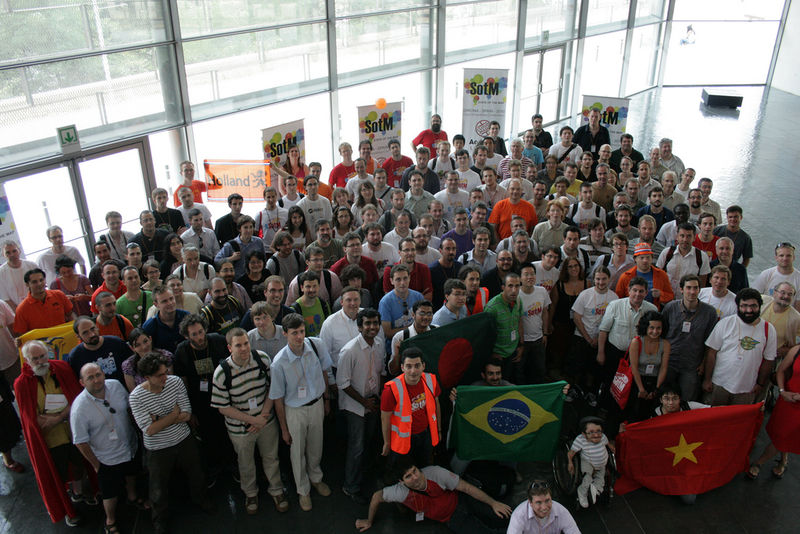
\includegraphics[width=5.5cm]{sotm.jpg}
 \end{center}

\end{frame}

%\begin{frame}{Wer steht hinter OpenStreetMap}
%
%  \begin{itemize}
%    \item OpenStreetMap Foundation (Server, Rechtliche Vertretung)
%      \pause
%    \item Mapper ($\sim$20.000 aktiv), meist ohne Geo-Hintergrund
%    \begin{itemize}
%      \item Jährliche Konferenz - "`State of the Map"', heuer: Buenos Aires
%    \end{itemize}
%      \pause
%    \item Universitäten
%    \begin{itemize}
%      \item Bakk-, Master- und Doktorarbeiten mit OSM
%      \item Server-Hosting
%    \end{itemize}
%      \pause
%    \item Organisationen, die Daten sponsern
%    \begin{itemize}
%      \item Firmen wie Yahoo/Bing, die Luftbilder zur Verfügung stellen
%      \item Regierungen mit besseren Open-Data-Gesetzen als Österreich %!!!!!!!!!!!!!!!!!!!!FIXME
%  % BSP TIGER, USA
%  % Dänemark, Hausnummern
%  % Frankreich,Tschechien: Kataster
%    \end{itemize}
%      \pause
%    \item Firmen die mit OSM arbeiten, z.B.:
%    \begin{itemize}
%      \item Geofabrik (de)
%      \item MapQuest (us)
%      \item BikeCityGuide (Graz)
%    \end{itemize}
%  \end{itemize}
%
%\end{frame}

  
%{
% \usebackgroundtemplate{\includegraphics[height=10cm]{Osmdbstats2_users.png}}
%
%\begin{frame}{Geschichte von OpenStreetMap}
%  \vspace{0.6cm}
%\begin{itemize}
%  \item Start des Projekts im August 2004 durch \emph{Steve Coast}
%  \item Dezember 2006 - Yahoo erlaubt abzeichnen
%  \item Juli 2007 - Erste Konferenz, "`State Of The Map"'
%  \item August 2007 - 10.000 Registrierte Benutzer
%  \item März 2009 - 100.000 Registrierte Benutzer
%  \item Januar 2010 - Haiti--Projekt
%  \item November 2010 - Bing erlaubt abzeichnen
%  \item Juli 2011 - Erste "`State Of The Map Europe"' in Wien
%  \item Januar 2013 - 1.000.000 Registrierte Benutzer
%  \item Gestern - 1.491.901 Registrierte Benutzer
%\end{itemize}
%
%\end{frame}
%}




\begin{frame}{Warum OpenStreetMap?}

\hspace{0.5cm}Es beginnt 2004 mit einer Geschichte: 
  \vspace{0.3cm}

Ein Student ärgert sich, dass es in UK keine freien Geodaten gibt. 
  \vspace{0.3cm}

\parbox{9.5cm}{Die Daten auf streetmap.co.uk wurden mit Steuergeldern erstellt, man kann die Rohdaten jedoch nicht frei verwenden.}
\hfill
\raisebox{\dimexpr-\height+\baselineskip}{
\includegraphics[height=1cm]{traurig.png}}

  \vspace{0.6cm}
\pause

Warum muss man für etwas, was bereits von der Allgemeinheit mit Steuergeld bezahlt wurde, nocheinmal bezahlen?
  \vspace{0.3cm}

\parbox{9.1cm}{Und darf es selbst dann nicht frei Nutzen? \\Doppelbesteuerung ist zumindest bei uns verboten?}
\hfill 
\raisebox{\dimexpr-\height+\baselineskip}{
\includegraphics[height=1cm]{grantig.png}}

\pause

 \parbox{7.5cm}{\vspace{0.4cm}\hspace{0.5cm}$\Longrightarrow$ \hspace{0.5cm}Er gründet OpenStreetMap!} 
\raisebox{\dimexpr-\height+\baselineskip}{
\includegraphics[height=1.2cm]{laugh.png}}

\end{frame}

\begin{frame}{Vision einer besseren Welt}

 Sollte es nicht so sein:
  \begin{itemize}
    \item Es gibt weltweit EIN Portal für ALLE Verwaltungs-Daten 
    \item In einheitlichem Format und Sprache
    \item Alte Versionen verfügbar (Um Änderungen zu verfolgen)
    \item Unkompliziert Fehler melden, oder selbst ausbessern kann
\pause
    \item Man keine Anträge stellen muss, sondern einfach einen Ausschnitt wählt und Rohdaten runterlädt
    \item Alle Daten unter einen freien Lizenz nutzen kann
  \end{itemize}

  \begin{columns}[c]
        \column{.5\textwidth}
        \begin{center}
  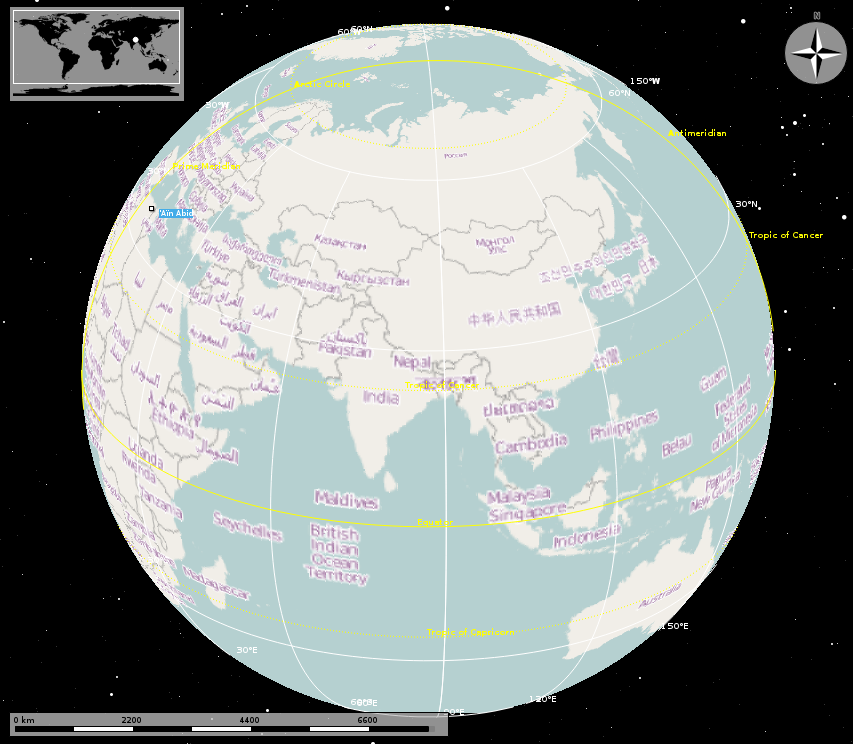
\includegraphics[width=3.5cm]{marble.png}
  \end{center}
        \column{.5\textwidth}
      \begin{center}
    
\includegraphics[width=2.5cm]{cc-by-sa.pdf}
  \end{center}
\end{columns}

\end{frame}


\section{Wie funktioniert OpenStreetMap?}

\begin{frame}{Woher kommen unsere Daten?}

\begin{itemize}
  \item Ursprünglich: GPS-Tracks
  \item Freiwillige tragen ihr Wissen bei: Jeder weiß viel über seine Umgebung:
	\begin{itemize}
	  \item Hausnummern, Straßennamen,
	  \item Restaurants, Bars, POIs, \dots
  \end{itemize}
  \pause
  \item Bei Mapping-Parties werden \\ gezielt Gebiete verbessert
\end{itemize}

  \vspace{0.4cm}
 99\% Handarbeit!

  \vspace*{-2.9cm}
 \hfill 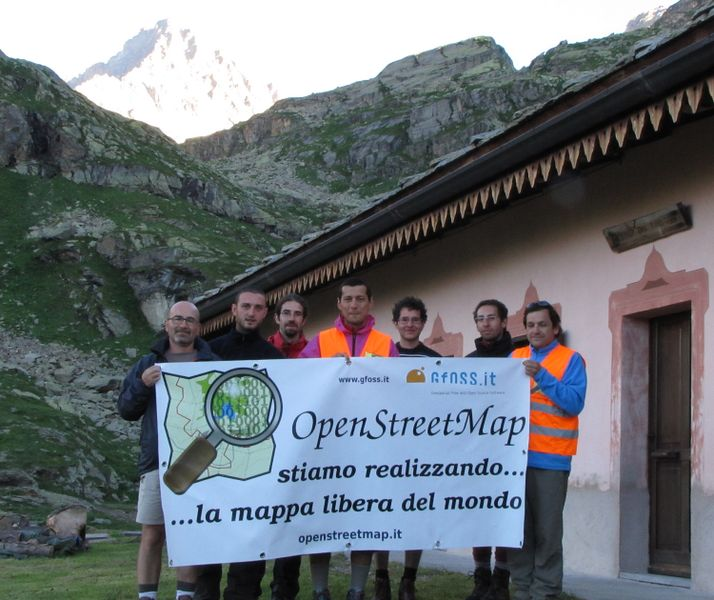
\includegraphics[width=4.2cm]{alps_mp.jpg}


  \pause
\begin{itemize}
  \item Unterstützt durch Open Government Data
  \begin{itemize}
    \item USA, TIGER Data (2008)
    \item Dänemark, Hausnummern (laufend synchronisiert)
    \item Graz, Steiermark, Wien, Engerwitzdorf... und 20 weitere
  \end{itemize}
\end{itemize}

\end{frame}

\section{OGD-Nutzung in OpenStreetMap}

\begin{frame}{OGD Graz in OpenStreetMap}
    
  \vspace*{-1.9cm}
 \hfill 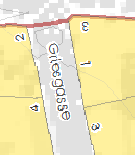
\includegraphics[width=3.0cm]{basiskarte.png}

  \vspace*{-2.0cm}
    Beispiel: Hausnummern

    \begin{itemize}
        \item Die Hausnummern sind auf der Grazer \\ Basiskarte 'analog' veröffentlicht
        \item Wir haben unsere fehlenden 35.000 mit \\ der Grazer Basiskarte ergänzt
  \vspace*{0.2cm}
        \item Damit wurden die Grazer Hausnummer weltweit durchsuchbar
        \item Werden in Navigationssystemen, zB BikeCityGuide genutzt
    \end{itemize}

  \vspace*{-0.7cm}
\begin{columns}[c]
\column{.5\textwidth}
\begin{center}
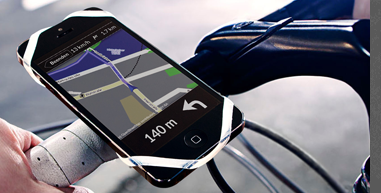
\includegraphics[width=4.5cm]{bcg.png}
\end{center}
\column{.5\textwidth}
\begin{center}
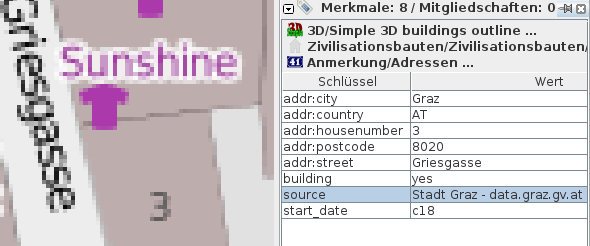
\includegraphics[width=5.5cm]{osm-gg3.png}
\end{center}
\end{columns}

\end{frame}
\begin{frame}{OGD Verbundlinie in OpenStreetMap}
    Beispiel: Haltestellen der Verbundlinie

    \begin{itemize}
        \item Haltestellen des Verkehrsverbundes Steiermark \\
            werden derzeit in die OpenStreetMap importiert
    \begin{itemize}
        \item $~$8.000/$~$16.000 schon importiert
    \end{itemize}
        \item Die nun öffentlichen Referenz- \\ nummern, z.B. "ref:IFOPT=\\at:46:4226:1:aus" können \\ für intermodales Routing \\ genutzt werden
  \vspace*{0.2cm}
        \item Bus/Bahn/Bim-Linien werden \\ importiert, daraus z.B. die \\ \href{http://ÖPNVkarte.de}{ÖPNVkarte.de} erstellt
  \vspace*{-4.3cm}
    \end{itemize}
 \hfill 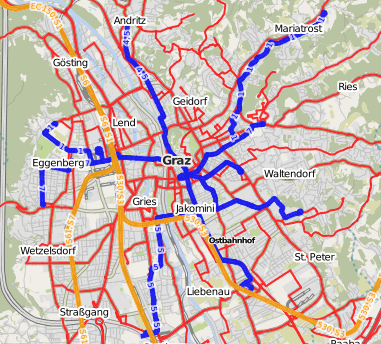
\includegraphics[width=5.0cm]{oepnv.png}

\end{frame}

\begin{frame}{OGD zur Qualitätssicherung in OpenStreetMap}
  Beispiel: Qualitätssicherung:
  \vspace*{0.2cm}

  Viele OGD-Veröffentlichungen werden zur Qualitätssicherung in der OpenStreetMap genutzt:
  \begin{itemize}
                  \item Apotheken und Krankenanstalten
                  \item Bibliotheken und Bildungsstandorte
                  \item Kinder- und Jugendorganisationen
                  \item Öffentliche Brunnen
              \end{itemize}
   Abgleich wurde in beide Richtungen durchgeführt:
  \begin{itemize}
                  \item Fahrradständer
                  \item Straßenverzeichnis
              \end{itemize}
                  
              Hier konnten als "`Rückfluss"' aus der Community fehlende / fehlerhafte Daten der Stadt Graz korrigiert werden

\end{frame}

\begin{frame}{OGD Visualisierung: Baumkataster}
    \href{http://www.opendatagraz.at/2014/06/23/grazer-baume/}{www.opendatagraz.at/2014/06/23/grazer-baume/}
    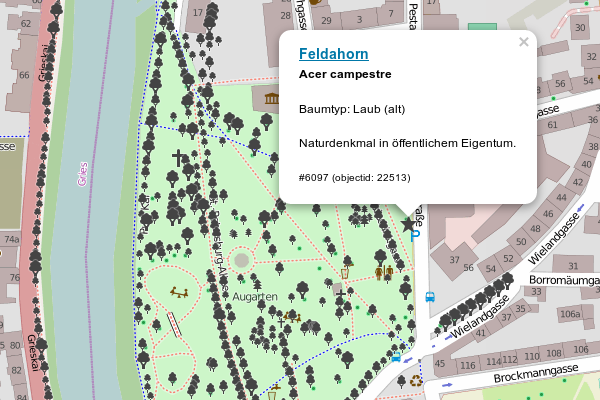
\includegraphics[width=10.0cm]{visualisierung-tyr.png}
\end{frame}
% 100% freie Software
% → jeder kann den Software-Stack verwenden http://openaviationmap.org/
% Quality Assurance
% * Es gibt automatische Q/A-Tools
% * kaum Streitfälle - wenn dann Mailinglist, Data Working Group
% * 
% tolle Bilder herzeigen!
% * irgendein Zoo
% * 3D -FIXME
% * Tolle Kartenstile:
%     * OSM-Fr?
%     * stamen watercolor
%     * pistemap
%     * bicycle map
%     * OpenSeaMap

% Wie daraus Karten generieren:
% 1F Toolchain
% nF Beispiele:
% * irgendein Zoo Mapnik -OK
% * 3D
% * Tolle Kartenstile:
%     * OSM-Fr? -OK http://tile.openstreetmap.fr/ -OK
%     * stamen watercolor -OK http://maps.stamen.com/watercolor/ -OK
%     * pistemap /snow http://www.opensnowmap.org/ -OK
%     * bicycle map -OK http://cyclemap.org/ -OK
%     * OpenSeaMap -OK http://openseamap.org/ -OOK
%   show http://toolserver.org/~osm/locale/ru.html
    

%
%\begin{frame}{Freie Datendaten ermöglichen freie Kartenstile}
%
%Der Standard-Kartenstil (Mapnik) ist auf \href{https://github.com/gravitystorm/openstreetmap-carto/}{Github} verfügbar
%\begin{itemize}
%  \item Kann für persönlichen Stil angepasst werden
%  \item Er wird kollektiv weiterentwickelt, jeder kann mitmachen!
%\end{itemize}
%
%\begin{center}
%\includegraphics[width=7cm]{style-mapnik.png}
%\end{center}
%
%\vspace{-0.5cm}
%weitere Stile: \url{http://wiki.osm.org/Featured\_tiles}
%
%\end{frame}
%
%\hypersetup{urlcolor=cyan}
%
%\begin{frame}{Französischer Stil:\hfill\url{http://tile.openstreetmap.fr/}}
%\begin{center}
%\includegraphics[height=7cm]{style-french.png}
%\end{center}
%\end{frame}
%
%\begin{frame}{Stamen Watercolor:\hfill\href{http://maps.stamen.com/watercolor/}{http://maps.stamen.com/watercolor}}
%\begin{center}
%\includegraphics[height=7cm]{style-stamen.png}
%\end{center}
%\end{frame}
%\hypersetup{urlcolor=blue}
%
%
%\hypersetup{urlcolor=cyan}
%
%\begin{frame}{Ski-Karte :\hfill\url{http://www.opensnowmap.org/}}
%\begin{center}
%\includegraphics[height=6.1cm]{style-snow.png}
%\end{center}
%\end{frame}
%
%\begin{frame}{See-Karte :\hfill\url{http://www.openseamap.org/}}
%\begin{center}
%\includegraphics[height=7cm]{style-seamap.png}
%\end{center}
%\end{frame}
%
%\begin{frame}{Fahrrad-Karte :\hfill\url{http://www.opencyclemap.org/}}
%\begin{center}
%\includegraphics[height=6cm]{style-cycle.png}
%\end{center}
%\end{frame}
%
%
%
%
%
%\section{OpenStreetMap Nutzen}
%
%
%\begin{frame}{Die Zukunft... 3D! }
%  Neu! Jetzt auch in 3D! Beispielsweise auf \href{http://maps.osm2world.org/?zoom=17&lat=47.06156&lon=15.46983&layers=BF0FTFFF}{maps.osm2world.org}.
%
%  \includegraphics[width=0.9\textwidth]{3d.png}
%
%
%\end{frame}
%
\begin{frame}{Hilfe}
Fragen? 
\begin{itemize}
  \item Dokumentation: \href{http://wiki.openstreetmap.org}{wiki.openstreetmap.org}
  \begin{itemize} 
    \item Mitmachen? \href{http://learnosm.org/}{learnosm.org}
  \end{itemize}
  \item Fragen stellen? \\ $\Rightarrow$ Mailingliste \href{http://lists.openstreetmap.org/listinfo/talk-at}{talk-at}
\vspace{1cm}
  \item Grazer \href{https://wiki.openstreetmap.org/wiki/Graz/Stammtisch}{Stammtisch}
  \begin{itemize}
      \item jeden 2. Montag im Monat 
      \item Brot $\&$ Spiele
  \end{itemize}

\end{itemize}

 \vspace*{-2.0cm}
\hfill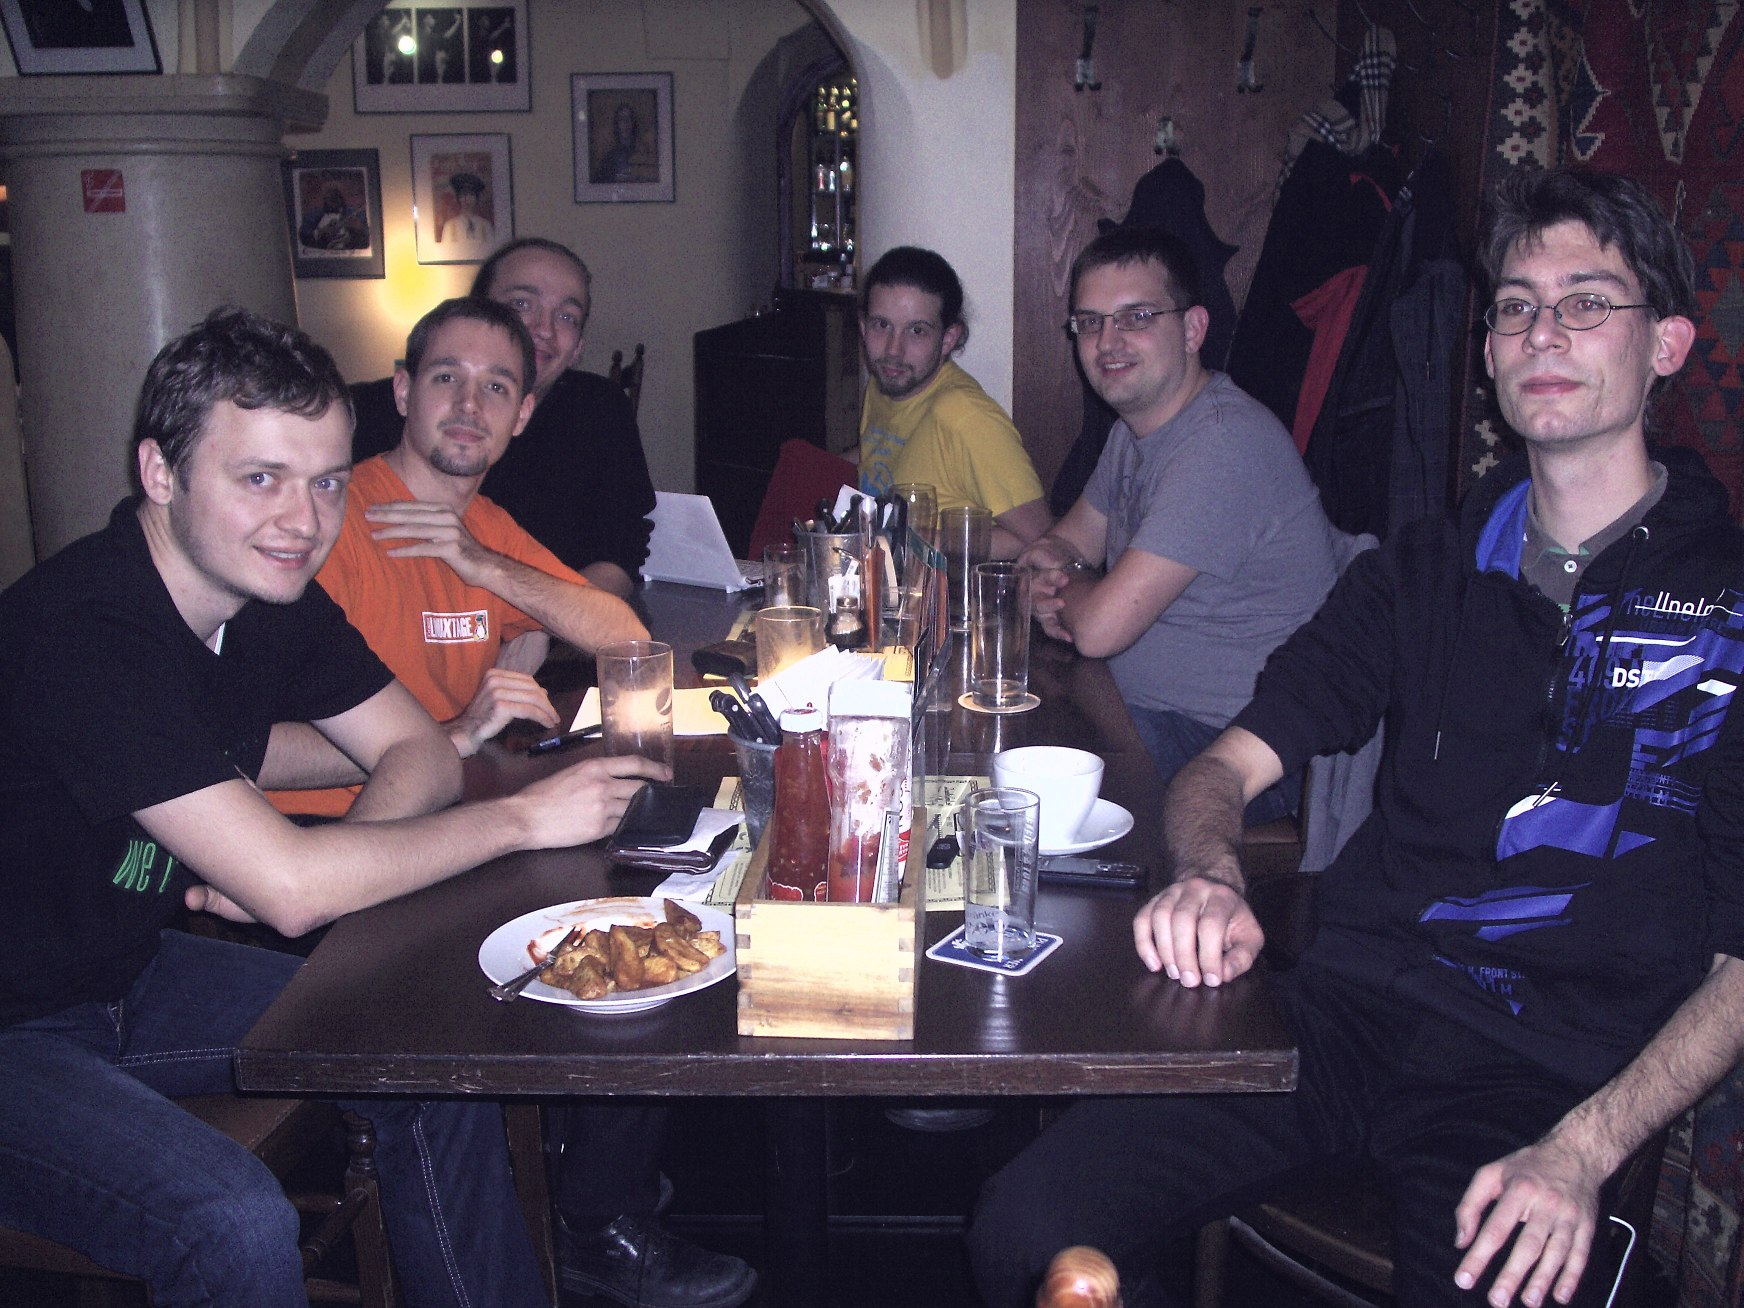
\includegraphics[width=5cm]{Osm_graz_members_2011.jpeg}

\end{frame}

\section{Ende}

\begin{frame}{Vielen Dank für die Aufmerksamkeit!}

  Folien zur OGD-Strategiegruppensitzung, 27.11.2014, Graz
\vspace{1cm}

Erstellt mittels \LaTeX Beamer, Quelltext: \href{https://github.com/species/vortrag-osm-ogdgraz}{Github}.
\vspace{1cm}

\href{mailto:michael.maier@student.tugraz.at}{Michael Maier}

Twitter: \href{https://twitter.com/osmgraz}{@osmgraz}
\vspace{1cm}

Folien unter: 
\includegraphics[width=1cm]{cc-by-sa.pdf}. 

Alle Daten ODbL, OpenStreetMap Contributors.

\end{frame}

\begin{frame}{Video: OSM Edits 2013}

  Video: "`A Year of Edits 2013"'

  \vspace{1cm}

\url{http://derickrethans.nl/year-of-edits-2013.html}  (2:06)

\vspace{1cm}

CC-BY-SA von Derick Rethans

\end{frame}

\end{document}
